\section{Trends and Analysis}
\subsection{Initial Constellation Tests} \label{sec:initial_constel}
During preliminary testing, a Molniya and Geosynchronous orbit were simulated. The results ruled them out as practical orbit options, restricting the bulk of study to LEO satellite constellations.
\subsubsection{Molniya Orbit}
A highly inclined molniya orbit was tested with orbital configuration such that the apogee\footnote{Point at which the satellite is farthest from the Earth} of the orbit occured over the LAX-Heathrow and LAX-Narita flight paths. The ground track of this orbit is shown in Figure \ref{fig:molniya}. It was observed that the satellite would `hang' for long periods of time over the apogee potentially allowing for a longer coverage time. Initial tests yielded a minimum received isotropic power of -161.985 dBW. This was more than 100 times weaker than the worst tested LEO constellation of -140.5 dBW.

\begin{figure}[H]
	\centering
	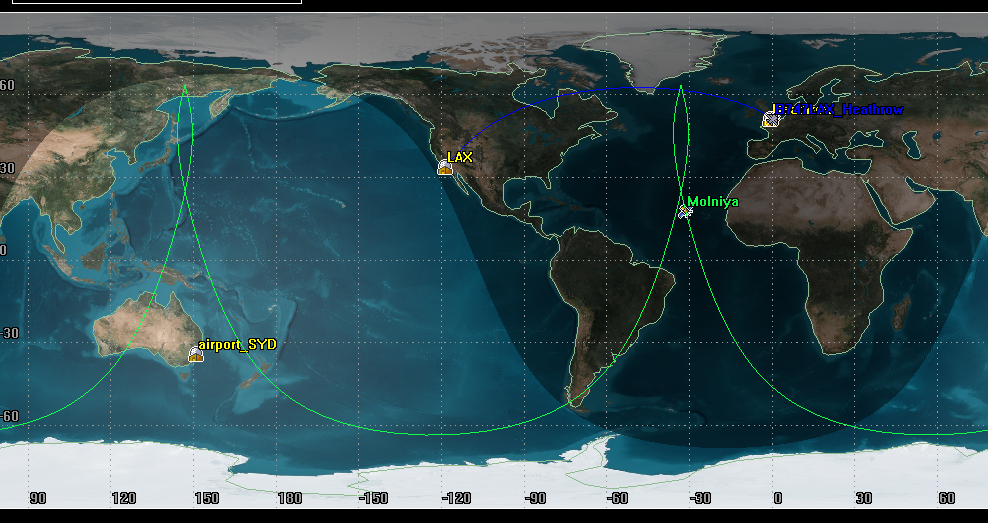
\includegraphics[scale = 0.50]{Pictures/molniya.png}
	
	\caption{Ground track of the tested Molniya orbit}
	\label{fig:molniya}
\end{figure} 

The access times for the LAX-Heathrow flight were evaluated by adding the additional constraint of having a minimum received isotropic power of at least 150.5 dBW (10 times weaker than the worst LEO constellation). This produced a coverage gap fraction of 0.992, meaning that the flight would spend more than 99 percent of the time not being able to communicate with an overhead satellite. This result and the poor signal performance resulted in the family of Molniya orbits being ruled out for further analysis.


\subsubsection{Geosynchronous}
A geosynchronus orbit with was tested with an inclination of 60 degrees and suborbital longitude of -30 degrees in order to place the ground track above the LAX-Heathrow flight. The ground track is given in Figure \ref{fig:geosynch}. The minimum received RX power ranged between -160.3 dBW in the best case and -161.69 in the worse case. This orbit was then dismissed because of the poor performing worst case signal when compared with LEO constellations. 

\begin{figure}[H]
	\centering
	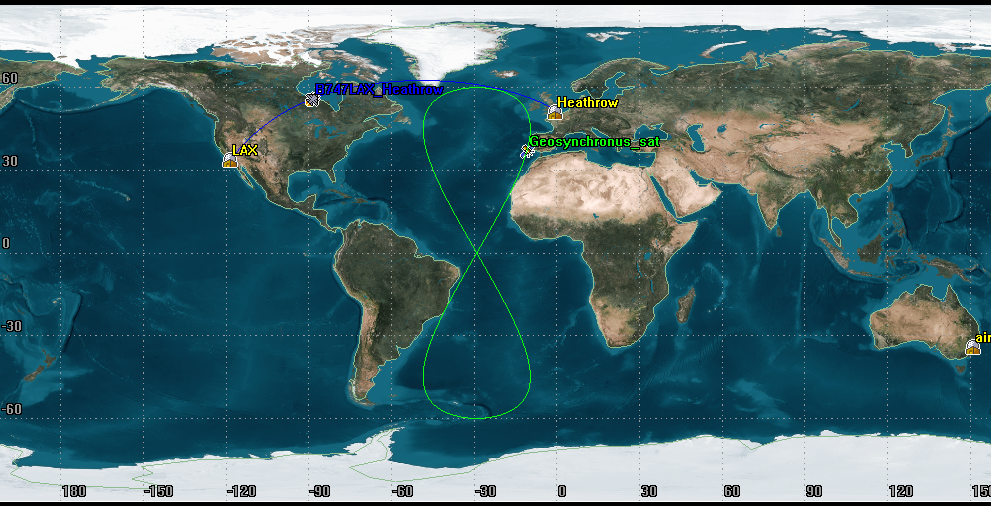
\includegraphics[scale = 0.55]{Pictures/geosynch.png}
	
	\caption{Ground track of the tested Geosynchronous orbit}
	\label{fig:geosynch}
\end{figure} 

\newpage
\subsection{Altitude Variations}
This series of tests involved evaluating the effect of uniformly changing the altitudes of each satellite from the reference case specified in Table \ref{tab:satRefCase} on the performance metrics outlined in Section \ref{sec:perfMetrics}.
\subsubsection{Input Variables}
From the reference case specified in Table \ref{tab:satRefCase}, the altitudes of each satellite were varied between 400km and 800km in 50km steps according to Table \ref{tab:altitudeParams}.

\begin{table}[H]
  \centering
  \caption{Altitude variations used}
    \begin{tabular}{p{2.5cm}rr}
    \toprule
    Case Number & Altitude (km) & Semi-Major Axis (km)\\
    \midrule
    1     & 400   & 6778.14 \\
    2     & 450   & 6828.14 \\
    3     & 500   & 6878.14 \\
    4     & 550   & 6928.14 \\
    5     & 600   & 6978.14 \\
    6     & 650   & 7028.14 \\
    7     & 700   & 7078.14 \\
    8     & 750   & 7128.14 \\
    9     & 800   & 7178.14 \\

    \bottomrule
    \end{tabular}%
  \label{tab:altitudeParams}%
\end{table}%
All other orbital parameters remained constant as per Table \ref{tab:satRefCase}.

It was originally thought that the high number of satellites in the reference constellation was causing a high degree of overlap between coverage from different satellites. This would pollute the observed trend of the access-coverage behaviour. The set of experiments was repeated using a smaller 3 satellite constellation with orbital parameters specified in Table \ref{tab:3sat_config}. The range of altitudes tested was the same as specified in Table \ref{tab:altitudeParams}.
% Table generated by Excel2LaTeX from sheet 'Sheet1'
\begin{table}[htbp]
  \centering
  \caption{Orbital parameters for 3 satellite test}
    \begin{tabular}{rrr}
    \toprule
    Satellite & RAAN  & True Anomaly \\
    \midrule
    1     & 0     & 0 \\
    2     & 120   & 120 \\
    3     & 240   & 240 \\
    \bottomrule
    \end{tabular}%
  \label{tab:3sat_config}%
\end{table}%



\subsubsection{Trends}
The results for altitude variations against the resulting coverage gap fractions, maximum gap period and minimum received signal power are shown in Figures \ref{fig:AltitudeVsCovGap12sat}, \ref{fig:AltitudeVsMaxGap12sat} and \ref{fig:AltitudeVsRxPower12sat} respectively. The results show that the coverage gap fraction and maximum coverage gap become lower with a higher satellite altitude. Similarly the minimum received isotropic power is reduced over time.  The coverage trends for the repeated three-satellite constellation test are given in Figures \ref{fig:AltitudeVsCovGap3sat} and \ref{fig:AltitudeVsMaxGap3sat}, showing the same trends.
\begin{figure}[htbp]
	\centering
	\includegraphics[scale = 0.6]{Pictures/AltitudeVsCovGap12sat.png}
	
	\caption{Coverage gap (as a fraction of total analysis time) as effected by altitude variations. Lower is better}
	\label{fig:AltitudeVsCovGap12sat}
\end{figure} 


\begin{figure}[htbp]
	\centering
	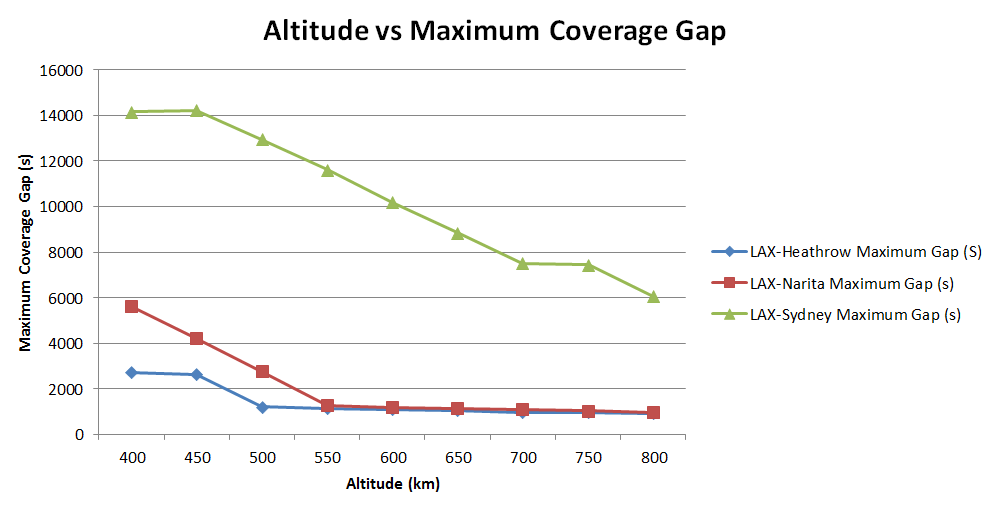
\includegraphics[scale = 0.6]{Pictures/AltitudeVsMaxGap12sat.png}
	
	\caption{Maximum coverage gap as affected by altitude variations. Lower is better}
	\label{fig:AltitudeVsMaxGap12sat}
\end{figure} 

\begin{figure}[htbp]
	\centering
	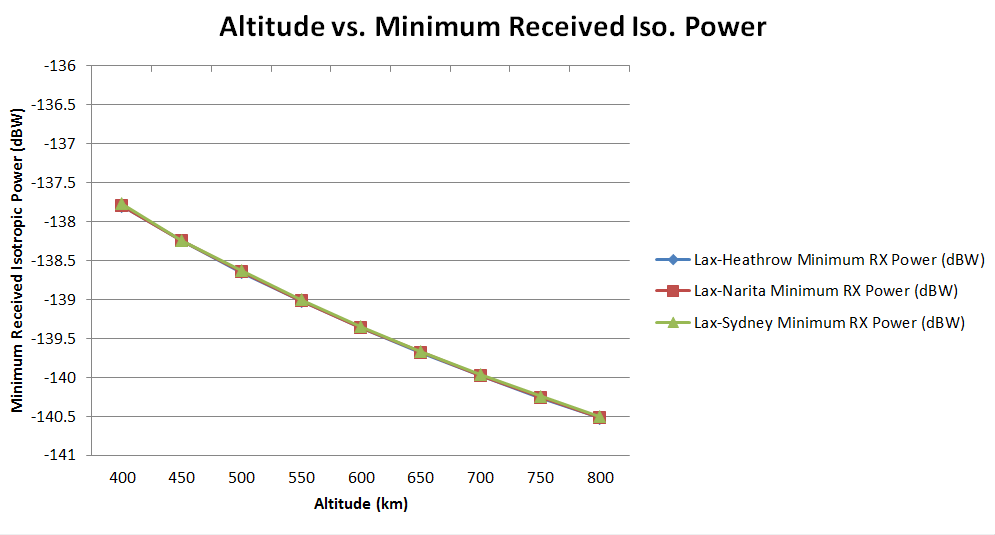
\includegraphics[scale = 0.6]{Pictures/AltitudeVsRxPower12sat.png}
	
	\caption{Minimum received isotropic power as affected by altitude variations. Higher is better.}
	\label{fig:AltitudeVsRxPower12sat}
\end{figure}


\begin{figure}[htbp]
	\centering
	\includegraphics[scale = 0.6]{Pictures/AltitudeVsCovGap3sat.png}
	
	\caption{Coverage gap (as a fraction of total analysis time) as effected by altitude variations with a 3 satellite constellation. Lower is better}
	\label{fig:AltitudeVsCovGap3sat}
\end{figure} 


\begin{figure}[htbp]
	\centering
	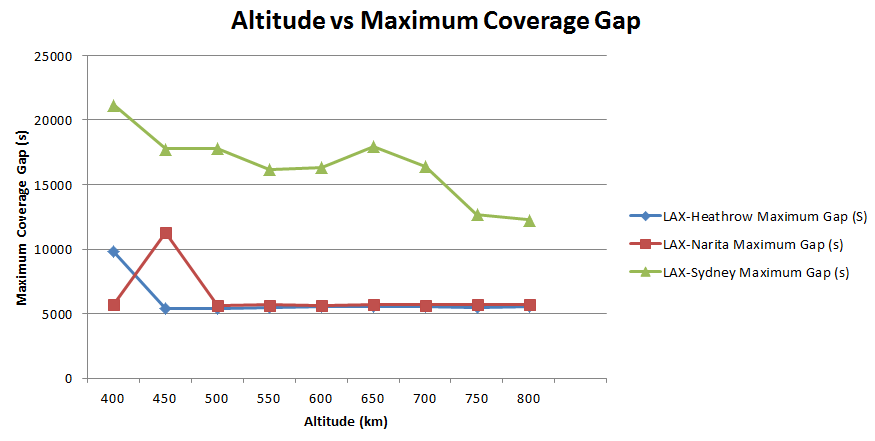
\includegraphics[scale = 0.6]{Pictures/AltitudeVsMaxGap3sat.png}
	
	\caption{Maximum coverage gap as affected by altitude variations retested with a 3 satellite constellation. Lower is better. }
	\label{fig:AltitudeVsMaxGap3sat}
\end{figure} 

\subsubsection{Discussion}
The results for both coverage gap times and received RF power behaved as expected. Satellites at higher altitudes have a greater line of sight range \footnote{The area on Earth within which objects will have a direct line of sight toward a satellite, allowing for a simple RF link to be made.} increasing the probability with which any one flight could be `seen' by a satellite. The difference in orbital period between the extremes of altitude (1 hour and 32.5 minutes at 800km against 1 hour and 42.9 minutes at 400 km) was less than 10\% and had minimal effect on the periodicity of access times. The net effect is the observed increase in coverage time and decrease of coverage `gaps' for any given flight path. The trends observed in the coverage-access times for the three-satellite test shown in Figures \ref{fig:AltitudeVsCovGap3sat} and \ref{fig:AltitudeVsMaxGap3sat} matched those quite closely with those seen in the reference case with 12 satellites. This indicated that the number of satellites did not affect the trend observed in either case

There was a significant observed difference in coverage gaps for the flights between LAX and Sydney and LAX and Heathrow or Narita. The maximum coverage gaps for LAX-Sydney were worse by one order of magnitude of time, as is shown in Figure \ref{fig:AltitudeVsMaxGap12sat}. This is due to the fact that 60 degree inclination of the satellites resulted in ground tracks that were almost coincident with the flight paths between LAX and Narita or Heathrow, as can be seen in Figure \ref{fig:12sat_60deg_flightPaths}. The geometry of the ground tracks was not optimised for the flight path between LAX and Sydney, resulting in a less desirable maximum coverage gap.

\begin{figure}[htbp]
	\centering
	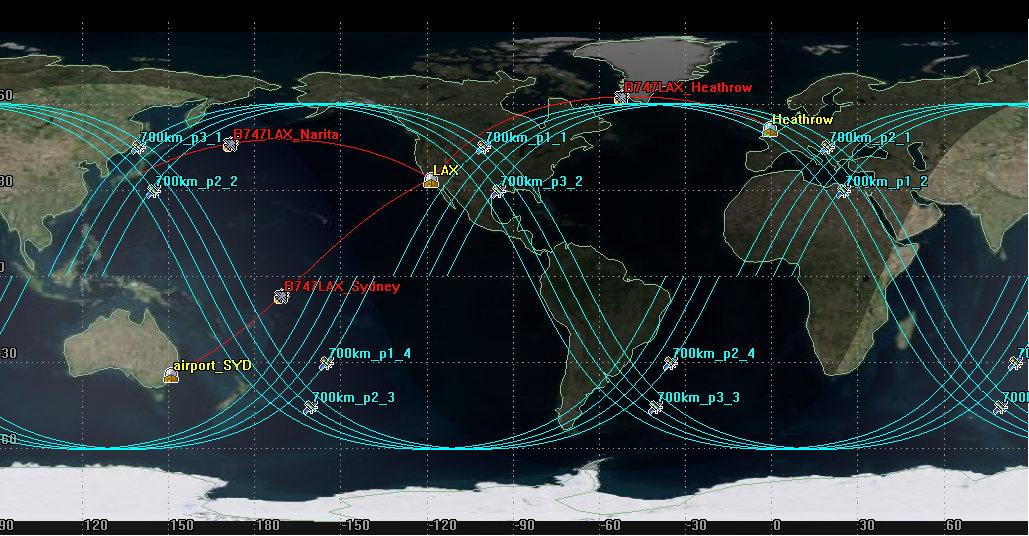
\includegraphics[scale = 0.6]{Pictures/12sat_60deg_flightPaths.png}
	
	\caption{Ground track of satellites inclined at 60 degrees, shown with the test flight paths}
	\label{fig:12sat_60deg_flightPaths}
\end{figure} 

Despite the increased access time at higher altitudes, however, a significant drop in received signal strength is observed between 400km and 800km altitude. There was an expected drop due to the increased distance and subsequent increased free-space path loss of any electromagnetic wave.  The minimum received isotropic power is optimised at 400km, with a measurement of -137.8 dBW and is the least optimised at 800km with a measurement of -140.5 dBW. This is a difference of 2.7 dBW, meaning that from 400km altitude to 800km altitude, the raw signal power has been reduced by a factor of 1.86. This will affect ADS-B detectability as weaker signals will be harder to detect and process. The effect of this on the performance of the system is evaluated later in Section \ref{sec:decision_matrix}.

The minimum trigger threshold level for an ADS-B receiver class R3 (Extended) as specified by the RTCA is set at -84 dBm \cite{RTCA_MODE_S} or -114 dBW. This is already well above that possible with the standard transmitter-receiver model at 400 km altitude. 


  
 
\newpage
\subsection{Inclination Variations}
This series of tests involved evaluating the effect of uniformly changing the inclination of each satellite from the reference case specified in Table \ref{tab:satRefCase} on the performance metrics outlined in Section \ref{sec:perfMetrics}.
\subsubsection{Input Variables}
From the reference case specified in Table \ref{tab:satRefCase}, the inclinations of each satellite were varied between 30 degrees and 90 degrees in 10 degree steps according to Table \ref{tab:inclinationParams}.

\begin{table}[H]
  \centering
  \caption{Inclination variations used}
    \begin{tabular}{p{2.5cm}r}
    \toprule
    Case Number & Inclination (degrees) \\
    \midrule
    1     & 30    \\
    2     & 40  \\
    3     & 60   \\
    4     & 70 	\\
    5     & 80    \\
    6     & 90   \\
    \bottomrule
    \end{tabular}%
  \label{tab:inclinationParams}%
\end{table}%
All other orbital parameters remained constant as per Table \ref{tab:satRefCase}. The ground tracks of the constellation inclined at 30 degrees, 60 degrees and 90 degrees is shown in Figures \ref{fig:12sat_30deg}, \ref{fig:12sat_60deg} and \ref{fig:12sat_90deg} respectively.
\begin{figure}[H]
	
	\begin{subfigure}[b]{\textwidth}
	\centering
	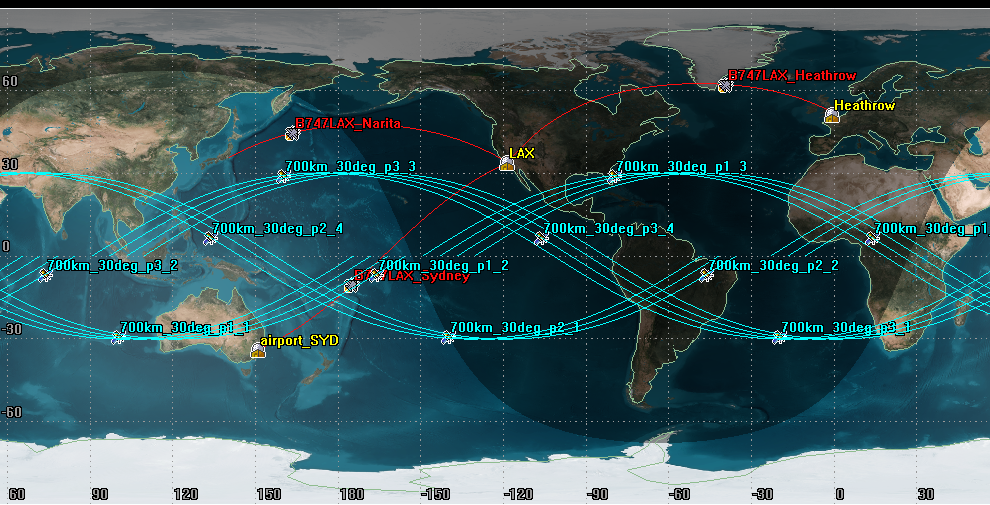
\includegraphics[scale = 0.45]{Pictures/12sat_30deg.png}
	
	\caption{Ground track of satellites inclined at 30 deg (Case 1)}
	\label{fig:12sat_30deg}
	\end{subfigure}
	
	\begin{subfigure}[b]{\textwidth}
	\centering
	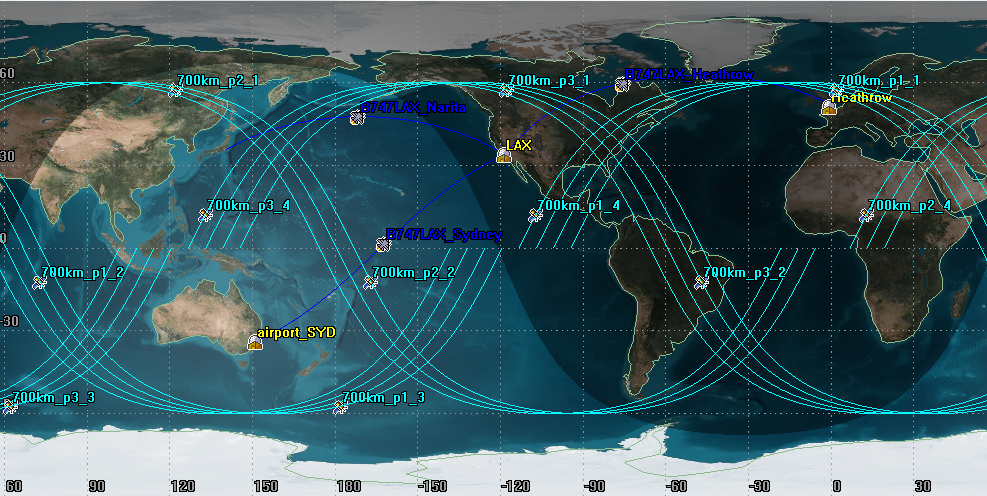
\includegraphics[scale = 0.45]{Pictures/12sat_60deg.png}
	
	\caption{Ground track of satellites inclined at 60 deg (Case 3)}
	\label{fig:12sat_60deg}
	\end{subfigure}
		
	
	\begin{subfigure}[b]{\textwidth}
	\centering
	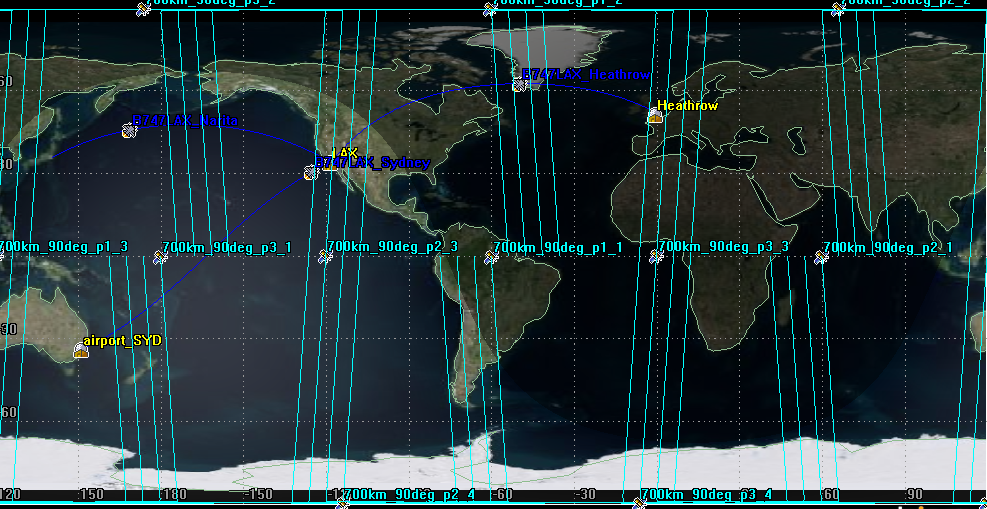
\includegraphics[scale = 0.45]{Pictures/12sat_90deg.png}
	
	\caption{Ground track of satellites inclined at 90 deg (Case 6)}
	\label{fig:12sat_90deg}
	\end{subfigure}
	
	\caption{Ground tracks of constellations inclined between 30 degrees and 90 degrees}
\end{figure} 

\subsubsection{Trends}
The results for inclination variations against the resulting coverage gap fractions, maximum gap period and minimum received signal power are shown in Figures \ref{fig:InclinationVsCovGap12sat}, \ref{fig:InclinationVsMaxGap12sat} and \ref{fig:InclinationVsRxPower12sat} respectively. Each parameter behaved differently for each flight.
\begin{figure}[htbp]
	\centering
	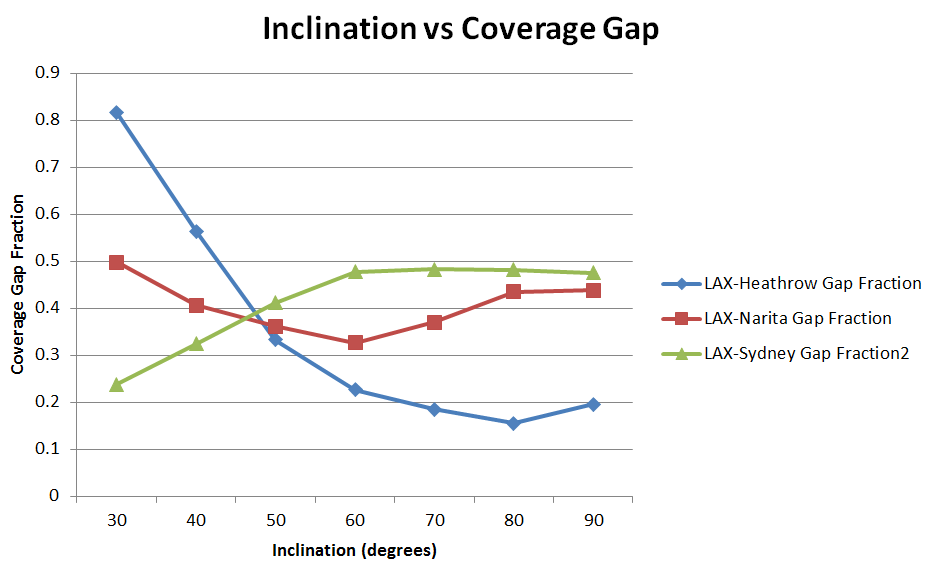
\includegraphics[scale = 0.6]{Pictures/InclinationVsCovGap12sat.png}
	
	\caption{Coverage gap (as a fraction of total analysis time) as effected by inclination  variations. Lower is better}
	\label{fig:InclinationVsCovGap12sat}
\end{figure} 


\begin{figure}[htbp]
	\centering
	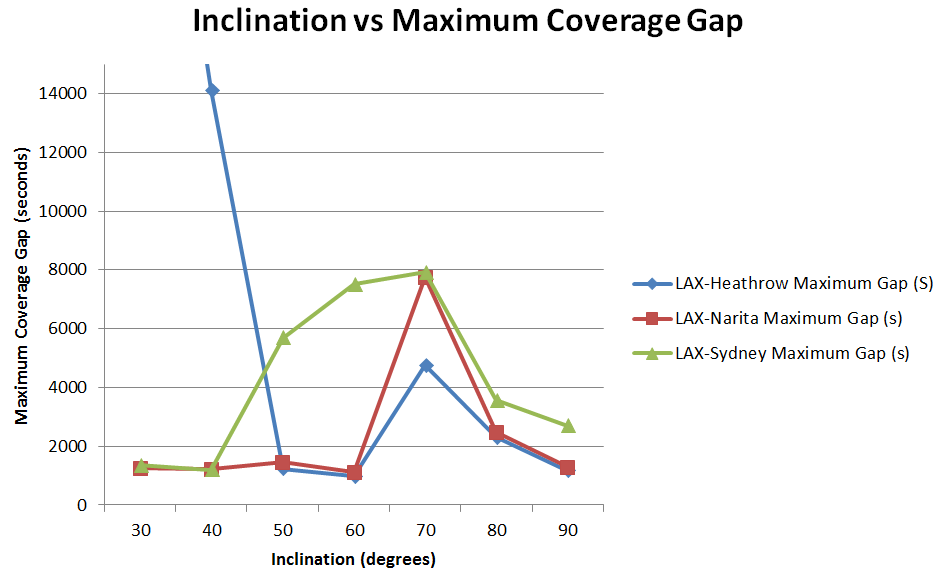
\includegraphics[scale = 0.6]{Pictures/InclinationVsMaxGap12sat.png}
	
	\caption{Maximum coverage gap as affected by altitude variations. Lower is better.}
	\label{fig:InclinationVsMaxGap12sat}
\end{figure} 

\begin{figure}[htbp]
	\centering
	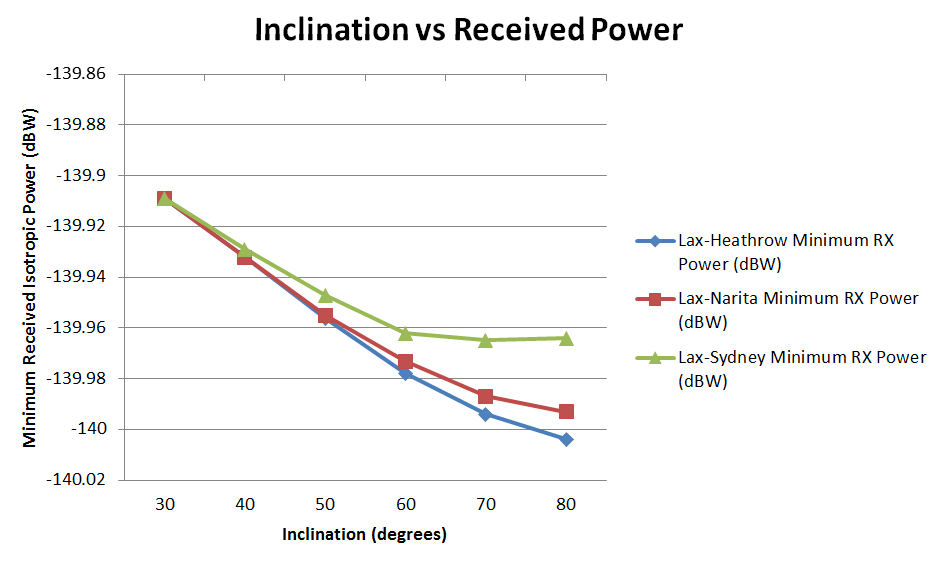
\includegraphics[scale = 0.6]{Pictures/InclinationVsRxPower12sat.png}
	
	\caption{Minimum received isotropic power as affected by inclination variations. Higher is better.}
	\label{fig:InclinationVsRxPower12sat}
\end{figure}
\subsubsection{Discussion}
At lower inclinations, the ground tracks of the satellite have a significant amount of coincidence with the flight path between LAX and Sydney, as seen in Figure \ref{fig:12sat_30deg}. This results in the LAX-Sydney flight path having an optimised maximum coverage time and coverage fraction at 30 degrees inclination as can be seen on Figures \ref{fig:InclinationVsCovGap12sat} and \ref{fig:InclinationVsMaxGap12sat}. Increasing inclinations resulted in a higher coverage gap ratio, before settling at 60 degrees and remaining constant through to 90 degrees.

The relatively high inclination of the LAX-Heathrow flight path resulted in poor coverage performance with the constellation at low inclinations. At low inclinations there were few opportunities for line of sight to be established between the LAX-Heathrow flight, with access periods only occurring when satellites reached high latitudes at the same time as the flight was at a low latitude. The resulting maximum gap (not shown in Figure \ref{fig:InclinationVsMaxGap12sat} for scale purposes) was 29 866 seconds (8 hours and 18 minutes) - more than half the duration of the flight. The aggregate result also yielded a poor coverage gap fraction performance below 50 degrees, as seen in Figure \ref{fig:InclinationVsCovGap12sat}. The effect sharply decreased with higher inclinations, with coverage gaps lowering to an acceptable level after 50 degrees.

All flight paths observed a spike in maximum coverage gap time with satellites inclined at 70 degrees, as seen in Figure \ref{fig:InclinationVsMaxGap12sat}. This occurred due to the geometry of the constellation and the effect of the Earth's rotation under the constellation. Figure \ref{fig:70_deg_precess_1_edited} shows that the effective width between the two orbital planes of the satellite is quite high, creating an effective radio `dead zone' in which the pictured plane cannot access a satellite. Although the plane continues to travel out of the `dead zone', the rotation of the Earth underneath the constellation moves the position of the plane back into the `dead zone', as demonstrated in  Figure \ref{fig:70_deg_precess_2_edited}. At inclinations of 80 degrees and 90 degrees this effect is mediated by the changing geometry and intersections between satellite ground tracks and flight paths, resulting in more acceptable coverage gaps.

There is relatively little change in the minimum received isotropic powers, with values ranging between -139.9 dBW and -140.02 dBW as seen in Figure \ref{fig:InclinationVsRxPower12sat}. The observed trend occurs due to the satellite having a higher chance of being `directly overhead' with higher inclinations, resulting in a shorted free-path propagation distance for the ADS-B signal. However this effect was quite small, only resulting in a net change of 0.12 dBW across the experimented range.

\begin{figure}[htpb]
	\centering
	\begin{subfigure}[b]{0.6\textwidth}
	
	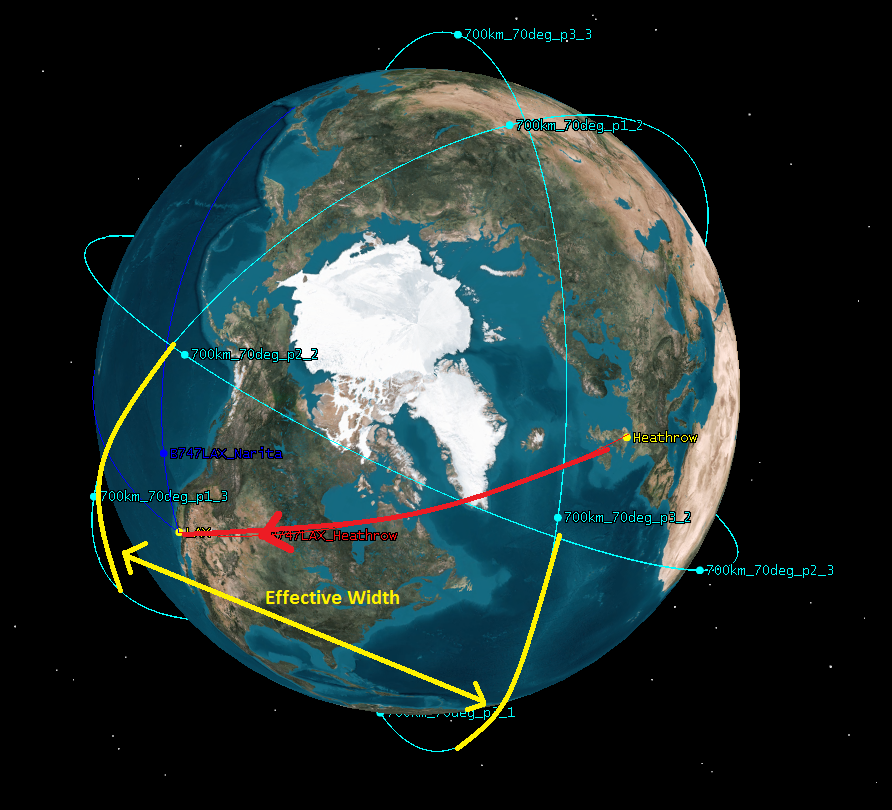
\includegraphics[width=\textwidth]{Pictures/70_deg_precess_1_edited.png}
	
	\caption{Flight initially in `dead zone' of no ADS-B access between planes}
	\label{fig:70_deg_precess_1_edited}
	\end{subfigure}
	
	\begin{subfigure}[b]{0.6\textwidth}
	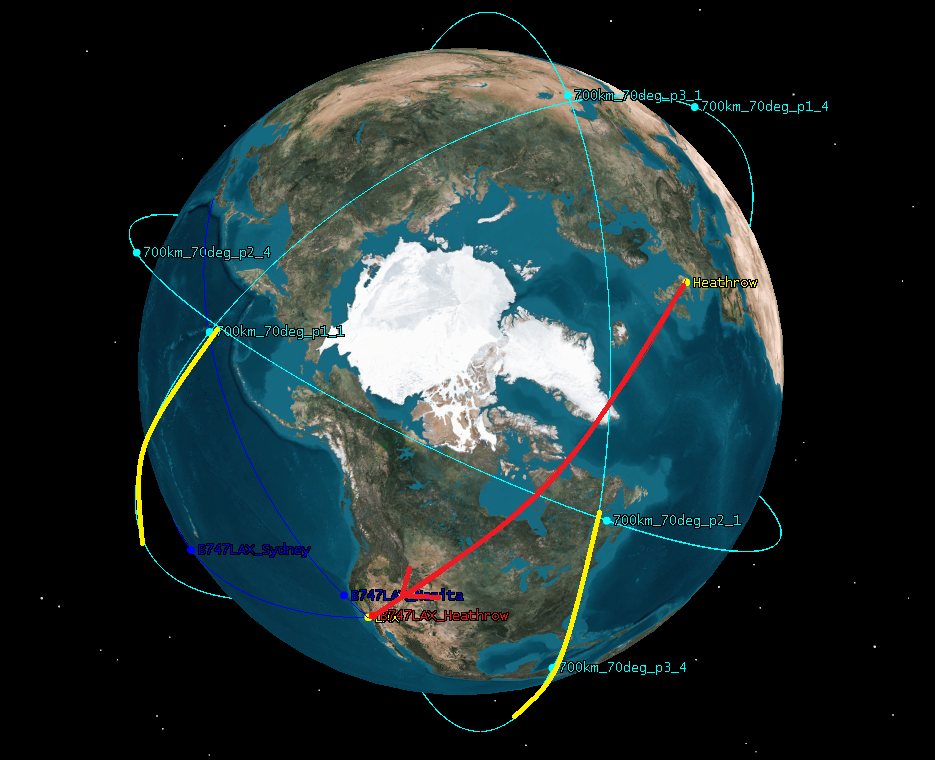
\includegraphics[width=\textwidth]{Pictures/70_deg_precess_2_edited.png}
	
	
	\caption{Rotation of Earth eastward keeps the flight in the `dead zone' for an extended period of time}
	\label{fig:70_deg_precess_2_edited}
	\end{subfigure}
		
	
	\caption{Flight in `dead zone' between satellite planes, inclined at 70 degrees. View from North Pole}
\end{figure} 
\newpage
\subsection{Satellite Number Variations}
This series of tests involved evaluating the effect of changing the number of satellites in the constellation on the performance metrics outlined in Section \ref{sec:perfMetrics}. The same three-plane orbital configuration was kept from Table \ref{tab:satRefCase}, whilst the number of satellites per-plane were changed. 
\subsubsection{Input Variables}
From the reference case specified in Table \ref{tab:satRefCase}, the number of satellites per each of the 3 planes were varied between 1 and 6 according to Table \ref{tab:perPlaneParams}.

\begin{table}[H]
  \centering
  \caption{Number of satellite variations used}
    \begin{tabular}{p{2.5cm}rr}
    \toprule
    Case Number & Satellites per plane & Total Satellites \\
    \midrule
    17    & 1     & 3 \\
    18    & 2     & 6 \\
    19    & 3     & 9 \\
    20    & 4     & 12 \\
    21    & 5     & 15 \\
    22    & 6     & 18 \\

    \bottomrule
    \end{tabular}%
  \label{tab:perPlaneParams}%
\end{table}%
All other orbital parameters remained constant as per Table \ref{tab:satRefCase}.

\subsubsection{Trends}
The results for satellite number variations against the resulting coverage gap fractions, maximum gap period and minimum received signal power are shown in Figures \ref{fig:PerPlaneVsCovGap12sat}, \ref{fig:PerPlaneVsMaxGap12sat} and \ref{fig:PerPlaneVsRxPower12sat} respectively. Generally it was seen that increasing the number of satellites per plane decreased the coverage gaps, whilst the minimum received RF power remained the same
\begin{figure}[H]
	\centering
	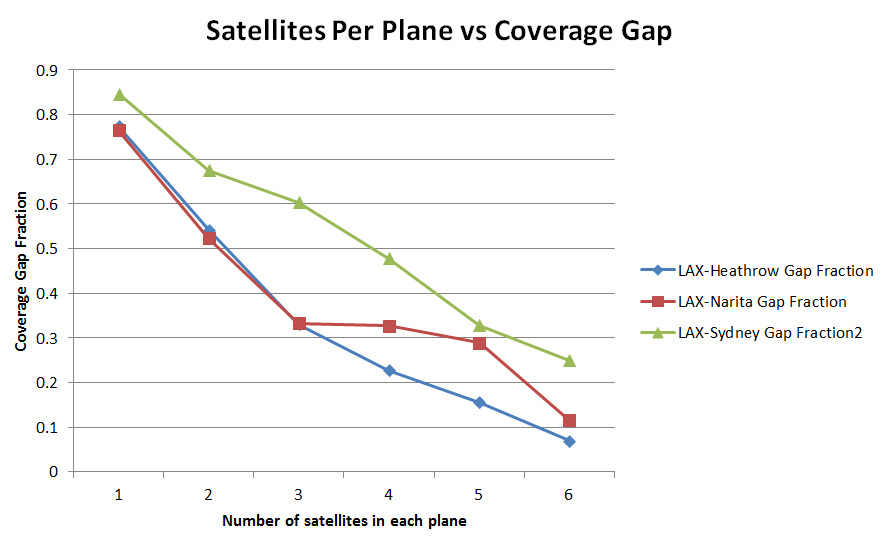
\includegraphics[scale = 0.6]{Pictures/PerPlaneVsCovGap12sat.png}
	
	\caption{Coverage gap (as a fraction of total analysis time) as effected by number of satellites per plane. Lower is better}
	\label{fig:PerPlaneVsCovGap12sat}
\end{figure} 

\begin{figure}[H]
	\centering
	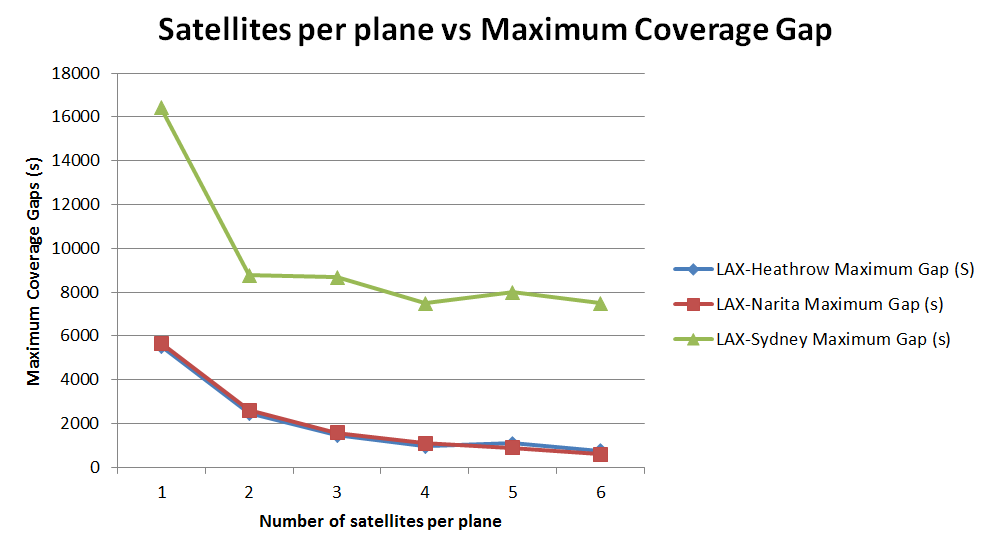
\includegraphics[scale = 0.6]{Pictures/PerPlaneVsMaxGap12sat.png}
	
	\caption{Maximum coverage gap as affected by number of satellites per plane. Lower is better.}
	\label{fig:PerPlaneVsMaxGap12sat}
\end{figure} 

\begin{figure}[H]
	\centering
	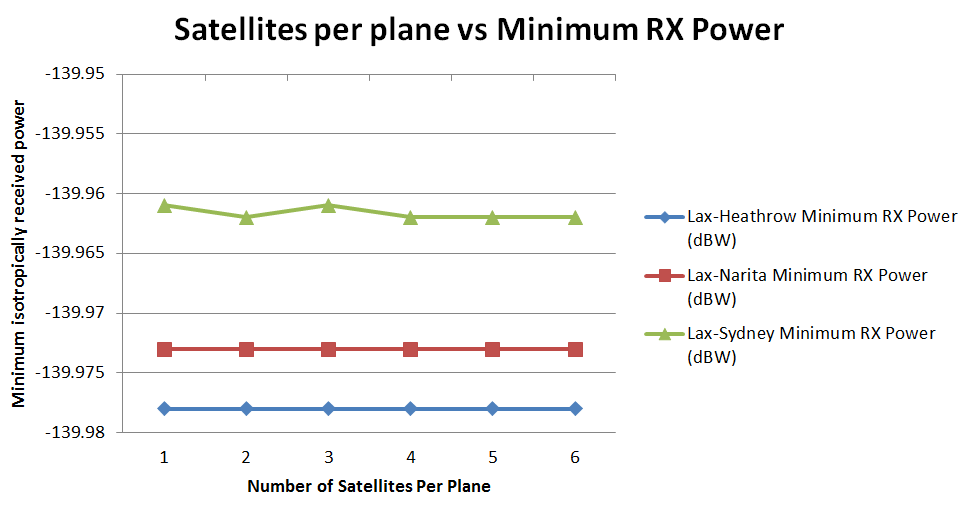
\includegraphics[scale = 0.6]{Pictures/PerPlaneVsRxPower12sat.png}
	
	\caption{Minimum received isotropic power as affected by number of satellites per plane. Higher is better.}
	\label{fig:PerPlaneVsRxPower12sat}
\end{figure}

\subsubsection{Discussion}
As expected, increasing the number of satellites increased the coverage times available for each flight. Figures \ref{fig:PerPlaneVsCovGap12sat} and \ref{fig:PerPlaneVsMaxGap12sat} show that a higher number of satellites results in less coverage gaps. A higher number of satellites per plane increased the probability with which a given flight was able to see at least one satellite, and also increased the revisit time for a given area on the Earth. The number of satellites in the constellation did not affect the minimum received RF power, as seen in the flatness of Figure \ref{fig:PerPlaneVsRxPower12sat}.

Despite the net beneficial effect on the ADS-B system, the number of satellites needs to be weighed against the cost and maintenance. Increasing the number of satellites did increase the effectiveness of the space based ADS-B coverage constellation. However a higher number of satellites will require an increased launch and maintenance cost, especially when considering the need to distribute the satellites evenly and potential replacement at end of life.


 

\section{Access Periodicity} \label{sec:periodicity_stats}
The distributions of coverage periods for all constellations tested were strongly modal, with the majority having one dominant mode. Figure \ref{fig:allfitdist_Heathrow}, from the reference constellation observing the LAX-Heathrow flight, shows a typical distribution. The periods shown all fall within a tight band around the mean, with some outliers and modes to the left and right of the mean. After applying \verb|allfitdist| \cite{sheppard12}, it was found that the Student's t distribution with a location and scale transformation applied, as shown in Figure \ref{fig:allfitdist_Heathrow}. An analysis of the Student's t distribution is given in Appendix \ref{sec:stats}.

\begin{figure}[htbp]
	\centering
	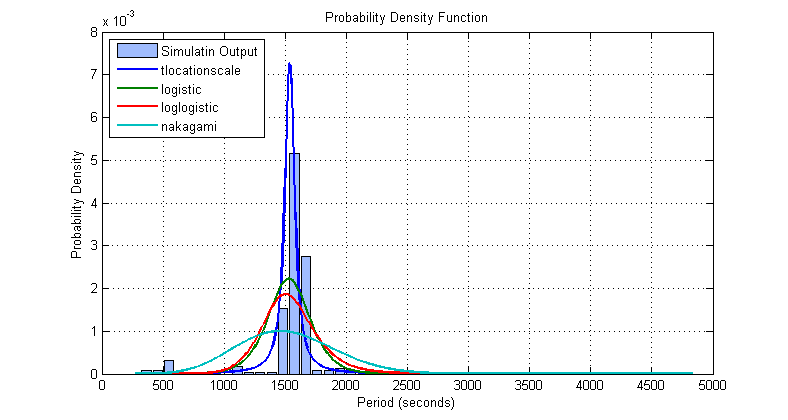
\includegraphics[scale = 0.85]{Pictures/allfitdist_Heathrow.png}
	
	\caption{Fitted distributions of the periodicity of Access times for the LAX-Heathrow flight from the reference constellation. }
	\label{fig:allfitdist_Heathrow}
\end{figure} 
For constellations with more than 12 satellites, the extracted parameters from \verb|allfitdist| yielded values for the degrees of freedom, $\nu$, for which the variance is undefined. Empirically, this was observed as the case if the band of most probable periods was too narrow for analysis using the Student's t distribution as the model. In these cases, the narrow variance was considered desirable and so for the purposes of comparative analysis, the `variance' score in the weighted decision matrix was given the highest score, 10.

It was found that for constellations with a lower number of satellites, there was less of a dominant node and more of an even spread of distributions. Figure \ref{fig:allfitdist_Heathrow6sat} shows the histogram for a six-satellite constellation, showing a larger spread of results. In these cases, \verb|allfitdist| yielded different distributions of best fit, as shown in Figure \ref{fig:allfitdist_Heathrow6sat}. Although these fits are not exact, the extracted variance value was considered a good indicator of comparative variance in periodicity. The standard deviations from these distributions were extracted computationally


\begin{figure}[htbp]
	\centering
	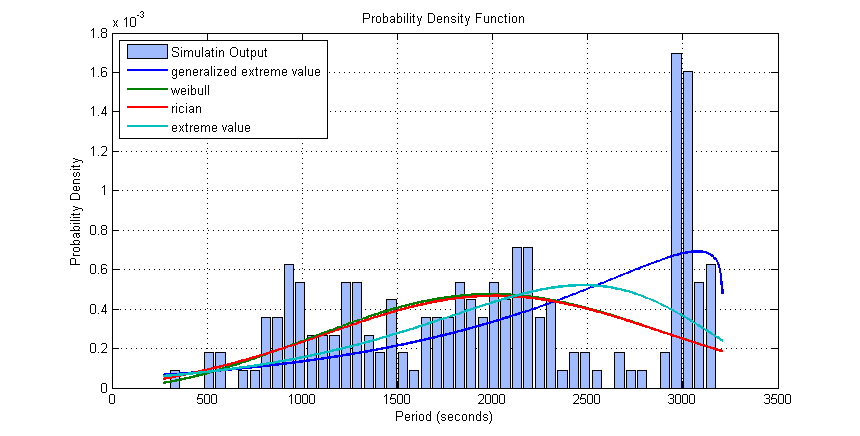
\includegraphics[scale = 0.8]{Pictures/allfitdist_Heathrow6sat.png}
	
	\caption{Fitted distributions of the periodicity of Access times for the LAX-Heathrow flight from the reference constellation. }
	\label{fig:allfitdist_Heathrow6sat}
\end{figure} 